\subsection{PWM Module Implementation}

PWM Module is implemented as in Exercise 3.

\subsection*{Simulation}

\textbf{PWM-Test 1} \hrulefill

In dieser PWM-Testbench wird der PWM-Generator statisch, ohne veränderung des
Duty-Cycles betrachtet. Zu sehen ist hier die Konfiguration
\lstinline{Period_counter_val_i = 1111} (15) mit dem
Arbeitszyklus\newline \lstinline{ON_counter_val_i = 0110} (6). Da der im
Zyklus der Wert 0 mit gezählt wird muss bei einer Periode vom 15 also von 0 bis
14 gezählt werden. Nun ist zu sehen, dass der Duty-Cycle von 6 genau sechs
Pulse der PWM Periode high ist.

\begin{center}
    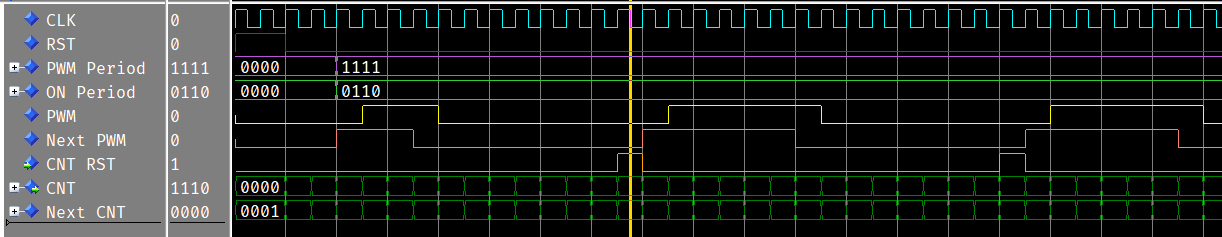
\includegraphics[width=1\linewidth]{images/SIM_PWM1.png}
\end{center}

